\documentclass[a4paper,9pt]{extarticle}

%=========================================================
% PACKAGES
%=========================================================

\usepackage[
a4paper,
top=1.8cm,
bottom=1cm,
left=1cm,
right=1cm,
headheight=14pt,
headsep=5mm
]{geometry}

\usepackage[T1]{fontenc}
\usepackage[utf8]{inputenc}
\usepackage[french]{babel}

\usepackage[sfdefault]{FiraSans}
\renewcommand{\familydefault}{\sfdefault}

\usepackage{multicol}
\setlength{\columnsep}{0.7cm}

\usepackage{amsmath,amssymb}
\usepackage{titlesec}
\usepackage{enumitem}

\usepackage{tcolorbox}
\tcbuselibrary{skins,breakable}

\usepackage{xcolor}
\usepackage{graphicx}
\usepackage{float}
\usepackage{tikz}

\usepackage{fancyhdr}
\usepackage[hidelinks]{hyperref}


%=========================================================
% PAGE SETTINGS
%=========================================================

\setlength{\parindent}{0pt}
\setlength{\parskip}{1.5pt}

\setlength{\abovedisplayskip}{4pt}
\setlength{\belowdisplayskip}{4pt}

\setlist[itemize]{
leftmargin=*,
itemsep=1pt,
topsep=1pt
}


%=========================================================
% COLORS
%=========================================================

\definecolor{Blue}{HTML}{E3F0FF}
\definecolor{Green}{HTML}{E3F7EA}
\definecolor{Pink}{HTML}{FFE5ED}
\definecolor{Orange}{HTML}{FFF0DC}
\definecolor{Purple}{HTML}{EEE7FF}
\definecolor{Yellow}{HTML}{FFFADB}

\definecolor{BlueTitle}{HTML}{285B8F}
\definecolor{GreenTitle}{HTML}{287052}
\definecolor{PinkTitle}{HTML}{A84063}
\definecolor{OrangeTitle}{HTML}{A96500}
\definecolor{PurpleTitle}{HTML}{6245A5}


%=========================================================
% HEADER
%=========================================================

\pagestyle{fancy}
\fancyhf{}

\fancyhead[L]{\small\textbf{Electronique I}}
\fancyhead[C]{\small Introduction au cours}
\fancyhead[R]{\small Week 01 -- 07-13/09/2026}

\renewcommand{\headrulewidth}{0.4pt}


%=========================================================
% TITLES
%=========================================================

\titleformat{\section}
{\large\bfseries\color{BlueTitle}}
{}{0pt}{}

\titlespacing{\section}
{0pt}{6pt}{3pt}


%=========================================================
% SEPARATOR
%=========================================================

\newcommand{\separator}{
\vspace{2pt}
\hrule
\vspace{3pt}
}


%=========================================================
% BOXES
%=========================================================

% DEFINITION - blue

\newtcolorbox{definition}{
enhanced,
breakable,
colback=Blue,
colframe=BlueTitle,
boxrule=0.7pt,
arc=0mm,
title=\textbf{Definition},
fonttitle=\bfseries
}


% IMPORTANT - pink

\newtcolorbox{important}{
enhanced,
breakable,
colback=Pink,
colframe=PinkTitle,
boxrule=0.7pt,
arc=0mm,
title=\textbf{Key idea},
fonttitle=\bfseries
}


% FORMULAS - green

\newtcolorbox{formula}{
enhanced,
breakable,
colback=Green,
colframe=GreenTitle,
boxrule=0.7pt,
arc=0mm,
title=\textbf{Key formulas},
fonttitle=\bfseries
}


% WARNING - orange

\newtcolorbox{warning}{
enhanced,
breakable,
colback=Orange,
colframe=OrangeTitle,
boxrule=0.7pt,
arc=0mm,
title=\textbf{Warning},
fonttitle=\bfseries
}


% EXAMPLE - purple

\newtcolorbox{example}{
enhanced,
breakable,
colback=Purple,
colframe=PurpleTitle,
boxrule=0.7pt,
arc=0mm,
title=\textbf{Example},
fonttitle=\bfseries
}


% SUMMARY - yellow

\newtcolorbox{summary}{
enhanced,
breakable,
colback=Yellow,
colframe=OrangeTitle,
boxrule=0.7pt,
arc=0mm,
title=\textbf{Summary},
fonttitle=\bfseries
}


%=========================================================
% DOCUMENT
%=========================================================

\begin{document}

\thispagestyle{fancy}

\footnotesize

\begin{multicols}{2}


%=========================================================
\section{Composants de base}


\begin{definition}

\textbf{Acquisition des informations}

Capteurs.

\textbf{Traitement des informations}

\begin{itemize}

\item conditionner le signal ;

\item l'analyser analogiquement ou numériquement.

\end{itemize}

\textbf{Reconditionner la solution}

\textbf{Actuateur}

Fournir l'information propre à un actuateur qui va agir sur son environnement.

\end{definition}



%=========================================================
\section{Opérateurs pour le choix d'une solution analogique ou numérique (peut aussi être hybride)}


\begin{example}

\centering

\textbf{Choix d'une solution numérique ou analogique}

\vspace{3pt}

\renewcommand{\arraystretch}{1.15}

\begin{tabular}{|p{0.42\linewidth}|p{0.42\linewidth}|}

\hline

\centering\textbf{Analogique}
&
\centering\textbf{Numérique}
\tabularnewline

\hline

Analyse
&
Portes logiques
\tabularnewline

\hline

Arithmétique
&
Logique combinatoire
\tabularnewline

\hline

Mise en forme de signaux :
amplifier, filtrer
&
Logique séquentielle
\tabularnewline

\hline

&
Machines d'états finis
\tabularnewline

\hline

&
Automates
\tabularnewline

\hline

&
Écriture d'algorithmes
\tabularnewline

\hline

\end{tabular}

\end{example}

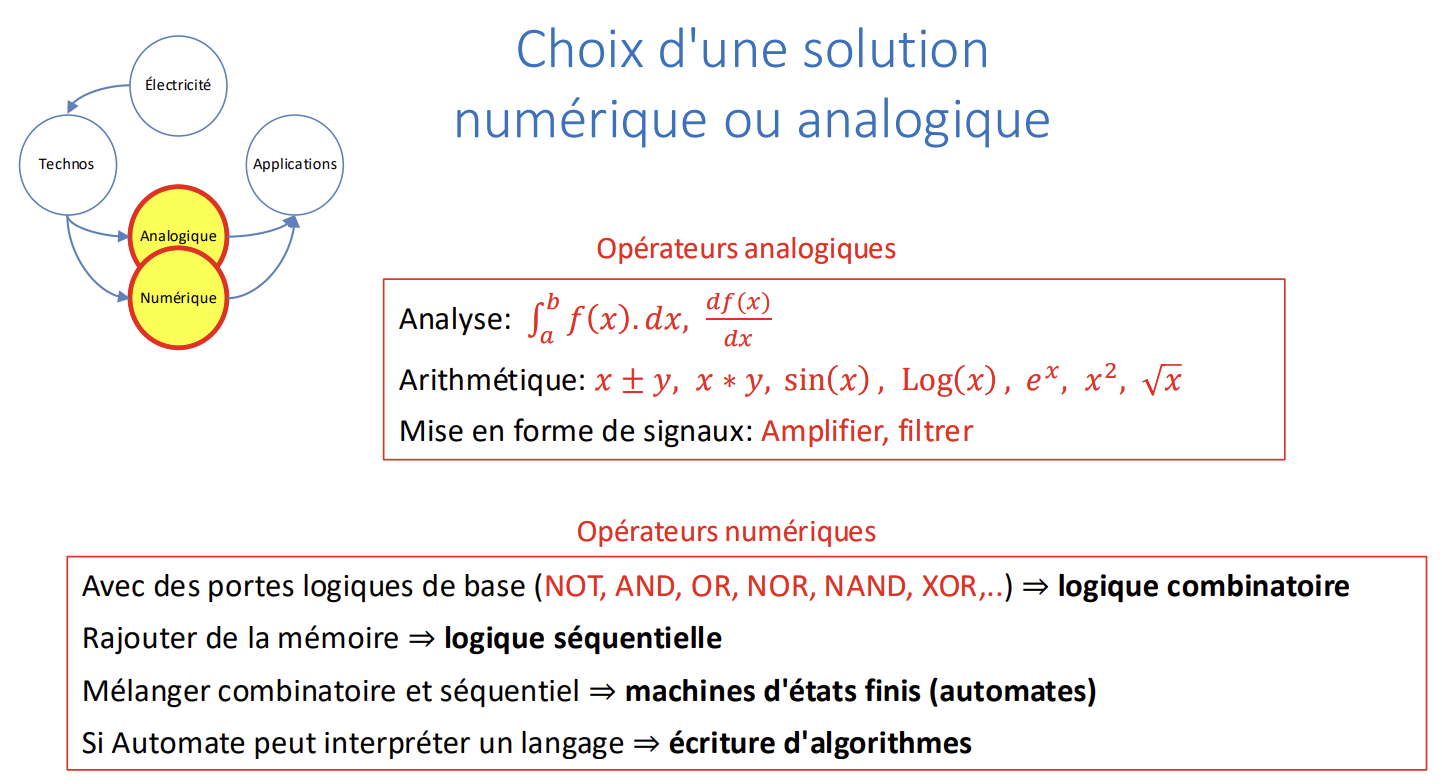
\includegraphics[
width=1.0\linewidth
]{../images/week01_01.png}



%=========================================================
\section{Avantages et inconvénients de l'analogique et numérique}


\centering

\textbf{Justification d'une solution numérique ou analogique}

\vspace{3pt}

\renewcommand{\arraystretch}{1.15}

\begin{tabular}{|p{0.42\linewidth}|p{0.42\linewidth}|}

\hline

\centering\textbf{Analogique}
&
\centering\textbf{Numérique}

\tabularnewline
\hline

\textbf{Avantages}
&
\textbf{Avantages}

\tabularnewline
\hline

Vitesse
&
Grande immunité au bruit

\tabularnewline
\hline

Respect du phénomène

(si le système est linéaire)
&
Transformation complexe avec peu de matériel

(algorithme)

\tabularnewline
\hline

Amplification du signal
&

\tabularnewline
\hline

\textbf{Inconvénients}
&
\textbf{Inconvénients}

\tabularnewline
\hline

Aucune immunité au bruit
&
Fréquences limitées

\tabularnewline
\hline

Transformation complexe avec beaucoup de matériel
&
Déformation du phénomène

\tabularnewline
\hline

&
Pas d'amplification du signal

\tabularnewline
\hline

\end{tabular}


%=========================================================
\section{Exemple : calcul de dérivée.................................................. }


\begin{example}

Les deux approches peuvent être utilisées.

\vspace{3pt}

\textbf{En analogique :}

Calcul de dérivée réalisé avec des AOP.

\vspace{3pt}

\textbf{En numérique :}

Échantillonnage et analyse de l'écart entre deux points.

\end{example}


\end{multicols}

\end{document}